\noindent
\textbf{RQ1}: \textit{How does our proposed approach perform compared to
the state-of-the-art?}




In this research question, we compare our two approaches \texttt{M1} (\ie{} neural network-based classification) and \texttt{M2} (\ie{} \rf{}-based classification), where both the models utilize GraphCodeBERT and Autoencoder to generate latent representation.
We compare the results from our models
against state-of-the-art approach from Aniche \etal{} \cite{Aniche2020Effectiveness}.
Though the baseline study compare many machine learning techniques,
we chose to compare our models with only their \rf{} model because it reported the best results in that study.
All of the models we tested using the same test split.
% as described in Section~\ref{dataset_prep}. 

\begin{table}[ht]
\centering
\caption{Experimental results for RQ1}
\label{tab:exresults}
\rowcolors{2}{gray!25}{white}
\begin{tabular}{p{4cm}|%
>{\raggedleft\arraybackslash}p{2cm}%
>{\raggedleft\arraybackslash}p{2cm}%
>{\raggedleft\arraybackslash}p{2cm}%
>{\raggedleft\arraybackslash}p{2cm}%
}
\textbf{Models} & \textbf{Accuracy} & \textbf{Precision} & \textbf{Recall} & \textbf{F1-score} \\ \midrule
M1 (GraphCodeBERT + Autoencoder + Neural Network) & $0.57$ & $0.71$ & $0.57$ & $0.63$ \\
M2 (GraphCodeBERT + Autoencoder + Random forest) & $\mathbf{0.87}$ & $\mathbf{0.90}$ & $\mathbf{0.87}$ & $\mathbf{0.88}$  \\
Baseline (with random forest) & $0.84$ & $0.44$ & $\mathbf{0.87}$ & $0.58$ \\\bottomrule
\end{tabular}
\end{table}


Table~\ref{tab:exresults} presents results of our experiments.
From the results it is evident that our \texttt{M2} model outperforms the baseline as well as the \texttt{M1} model. 
We observe that both \texttt{M1} and \texttt{M2} outperform the baseline. Specifically, we see that \texttt{M2} outperform the \rf{} used by Aniche~\etal{} by nearly 50\% in terms of precision.
At the same time, our model \texttt{M2} exhibits a good recall rate of $0.87$.
Consequently, we see that our model 
performs significantly better than the considered baseline model by approximately $30\%$ in terms of F1 score.


\begin{boxH}
\textbf{RQ1 Summary:} 
Our results show that our \rf{}-based model outperforms the baseline model significantly (by $30\%$, in terms of F1 score).
The results indicate that our  code representation is successfully capturing syntactic and semantic characteristics of code necessary to identify \exm{} refactoring candidates.
\end{boxH}

\noindent
\textbf{RQ2}: \textit{How effectively does the autoencoder extracts features for the classification task?}
% \vspace{0.3mm}

We train an autoencoder model and use the trained encoder part of it as a feature extractor.
We do so to reduce the vectors' dimensionality and extract relevant features from the embeddings generated from \GCB{}. 

\begin{figure}[htbp]

\begin{minipage}[t]{0.49\linewidth}
    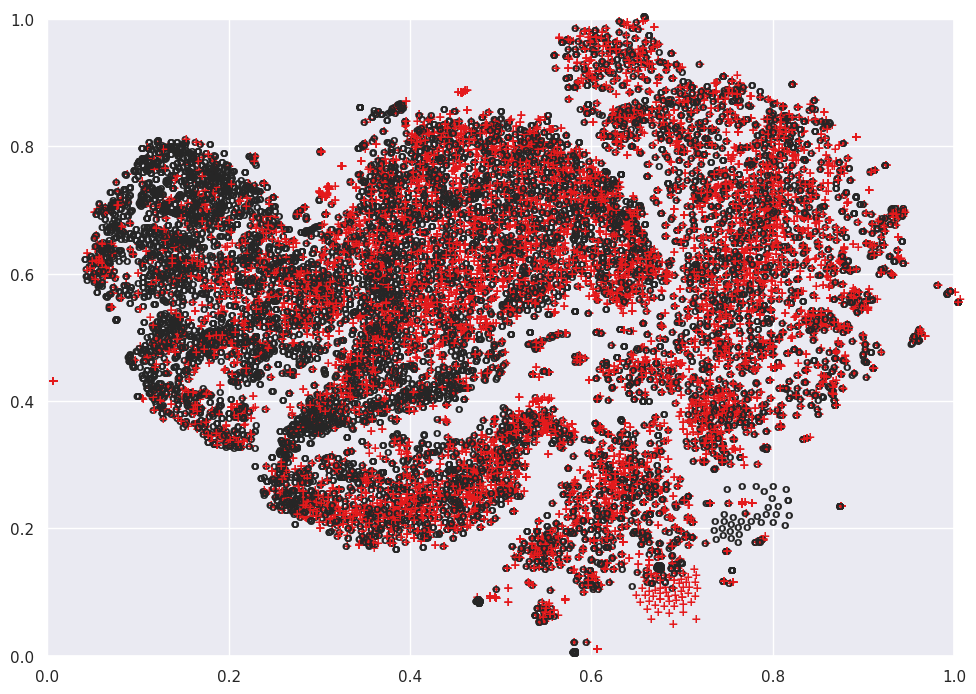
\includegraphics[width=\linewidth]{chapters/identification/Images/tsne_gc.png}
    \caption{Class separation with embeddings (from \GCB{})}
    \label{embonly}
\end{minipage} 
    \hfill%
\begin{minipage}[t]{0.49\linewidth}
    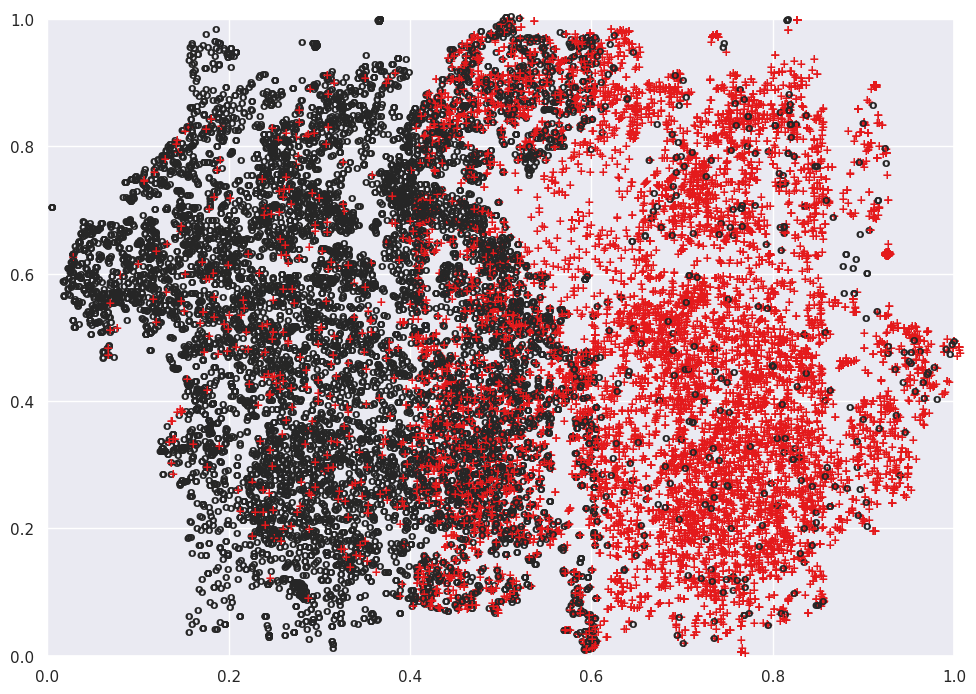
\includegraphics[width=\linewidth]{chapters/identification/Images/tsne_ae_1.png}
    \caption{Class separation with encoded embeddings (from Autoencoder)}
    \label{encodedemb}
\end{minipage}%

\end{figure}


% As we can see from the curve, the model performs well at reconstructing the input embeddings with minimum loss. 
To measure the performance and usefulness of the trained autoencoder model as a feature extractor, we first analyze the \texttt{t-SNE}~\cite{van2008visualizing} plots of the embeddings generated by \GCB{} and those generated by the combination of \GCB{} and Autoencoder. We do so to study the class separability. The distinguishability of classes in the \texttt{t-SNE} space is assessed through a clear separation and quantified by calculating the Euclidean distance between the centroids of each class. Figure~\ref{encodedemb} shows a reasonably clear bifurcation between the classes with an euclidean distance of $0.367$ as compared to $0.122$ for Figure~\ref{embonly}. We can infer that a classification model trained on the encoded embedding will perform better than the one trained on embeddings alone. This observation can be attributed to the autoencoder being able to learn hidden features unique to each type of sample which helps it to segregate them.

To further investigate the effectiveness of these representations, we perform an ablation study where we train classifier with and without the autoencoder representation of the embeddings. 
% In the first case, we train and test the model directly with the embeddings generated by \GCB{}. 
% In another case, after generating the initial embeddings for the training set from \GCB{}, we encode them using the trained encoder part of the autoencoder model. 
We report the performance results in Table~\ref{tab:emcomp}.
% The evaluation metrics are computed and reported in Figure~\ref{fig:aechart} for a comparative analysis. 
The \rf{} classification model, when trained with the encoded representation of the embedding provided by Autoencoder, 
outperforms the one trained with only the \GCB{} embedding vector as features. 
% While we observe a slight increase of \textbf{$7\%$} in terms of Precision metric value, there's a significant increase of about \textbf{$28\%$} on average for the other 3 metrics. 
These findings support our claim that the
autoencoder extracts features and reduces dimensionality effectively
in the context of refactoring candidate identification.

\begin{boxH}
\textbf{RQ2 Summary:} Autoencoder-encoded code representations from \GCB{} significantly improve classification performance compared to \GCB{} representations alone.
\end{boxH}


\begin{table}[h!]
\centering
\caption{Encoded embedding performance}
\label{tab:emcomp}
\rowcolors{2}{gray!25}{white}
\begin{tabular}{p{4cm}|%
>{\raggedleft\arraybackslash}p{2cm}%
>{\raggedleft\arraybackslash}p{2cm}%
>{\raggedleft\arraybackslash}p{2cm}%
>{\raggedleft\arraybackslash}p{2cm}%
}
\textbf{Models} & \textbf{Accuracy} & \textbf{Precision} & \textbf{Recall} & \textbf{F1-score} \\ \midrule
\begin{tabular}[c]{@{}l@{}}Embeddings\end{tabular} & $0.57$ & $0.71$ & $0.57$ & $0.63$ \\
\begin{tabular}[c]{@{}l@{}}Encoded embeddings\end{tabular}  & $\mathbf{0.87}$ & $\mathbf{0.90}$ & $\mathbf{0.87}$ & $\mathbf{0.88}$ 
% Baseline (with random forest) & 0.84 & 0.44 & \textbf{0.87} & 0.58
\\\bottomrule
\end{tabular}
\end{table}